\chapter{Tarkvaratehnika}
\section{Kokkuhoiust programmeerijatelt}
\label{sec:kokkuhoid}
Joel ütleb õigesti, et programmeerijate arendamiselt kokku hoida ei ole mõistlik. Sama kehtib ka teiste valdkondade inimeste puhul, kuid programmerijate töö on teiste omast suhteliselt info- ja teadmismahukam.

Valest kohast kokku hoitud raha (või värbamisel tehtud vead) võivad viia järgmise tagasisideni (vt. joonis \ref{fig:kokkuhoid}\footnote{Pluss-märk noolel ei tähenda mitte positiivset mõju vaid seda, et muutujad liiguvad samas suunas: ühe tõusule järgneb teise tõus ja langusele langus}):
\begin{enumerate}
	\item Koodi kvaliteet on madal
	\item Mistõttu kulub suhteliselt rohkem raha vigadega tegelemiseks ja teenitakse vähem
	\item Mis viib alla ettevõtte võimekuse inimestesse investeerida
	\item Mispeale langeb inimeste kompetentsitase veelgi (tehnoloogia ju areneb)
	\item Madalad kompetentsid viivad aga madalale koodi kvaliteedi
\end{enumerate}

Eesti IT-ettevõtted jagunevad ITLi andmetel suhteliselt radikaalselt kaheks: suured ning kasumlikud ning väikesed ja virelevad. Seda veelahet võib seletada läbi selle, kellel on õnnestunud tsükkel mis pidi tööle panna sest, muidugi, kehtib ka vastupidine. Kõrge koodi kvaliteet viib suuremate sissetulekuteni jne.

\begin{marginfigure}
		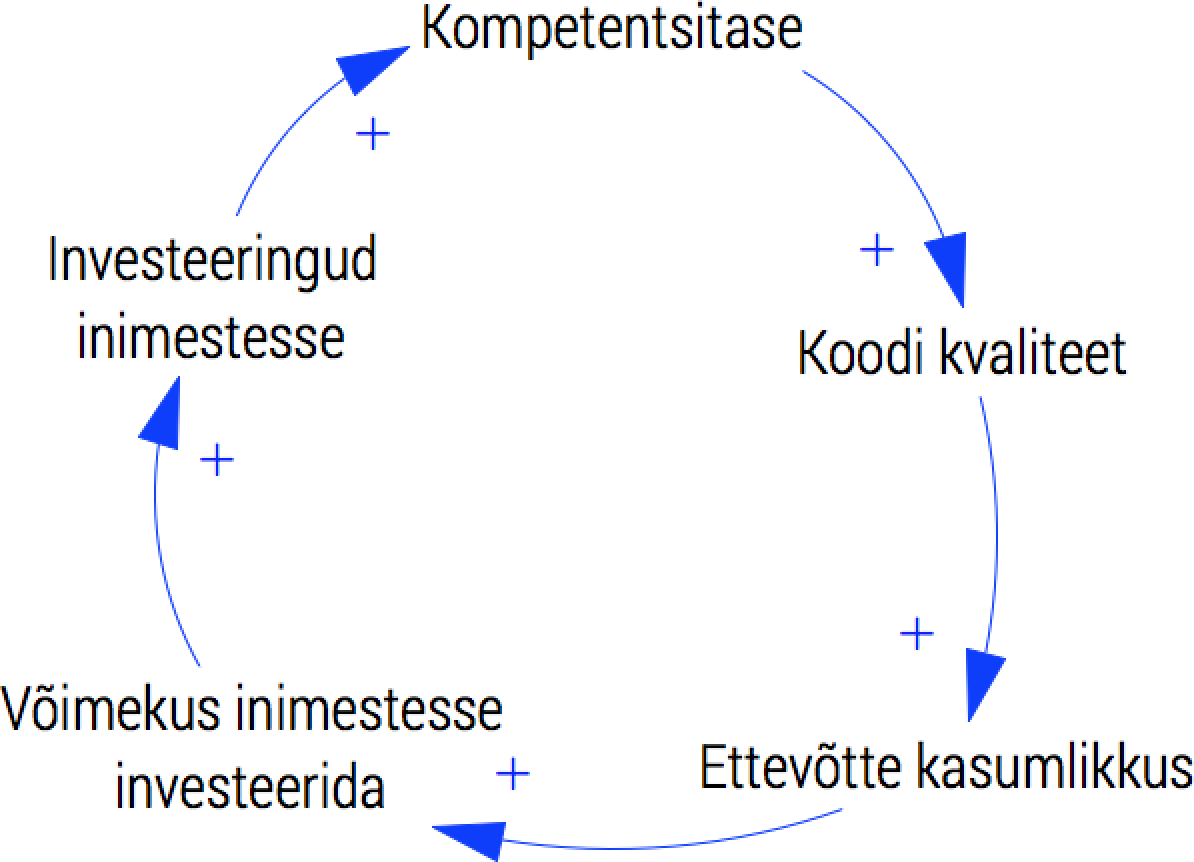
\includegraphics[width=\linewidth]{kvaliteet.png}
		\caption{Kompetentside ja kokkuhoiu seos tagasisides}
		\label{fig:kokkuhoid}
\end{marginfigure}

\section{Kood ei roosteta. Või siiski?}
\label{sec:rooste}
Joel Spolsky\index{Spolsky, Joel} ütleb, et reeglina on väga halb mõte oma koodibaasi ümber kirjutada, sest kood ju "ei roosteta" \citep{joelrust}. Ta toob mitu näidet väga ebameeldivate tagajärgedega ümber-kirjutamis ettevõtmiste kohta ning, tõesti, neid on ka siinkirjutaja praktikas mitmeid ette tulnud. Põhjuseid on mitmeid, peamiseks ehk paratamatu teadmuskadu: iga tükki koodi on juba enne rakenduse valmimist kümneid kui mitte sadu kordi muudetud ja parandatud\sidenote{Seejuures parandatud vigu me teame. Aga mis saab vigadest, mida kunagi eri raporteerita, millest me definitsiooni järgi midagi ei tea kuid millega kasutajad ja partnerid elama on õppinud?} parandamaks vigu, ületamaks nõuete ebatäielikkust jne. Nii kaob igasugune võimalus hinnata, kas kood on selline, nagu ta on, põhjusega või põhjuseta. Rääkimata analüüsist, kas põhjus jätkuvalt kehtib. Miks siis tekib vahel siiski kihu asju ümber teha ning miks on Eestis kehtestatud \emph{no legacy policy}?

Ühest küljest on asja taga kindlasti programmeerijad. Nagu Spolsky õigesti osundab, on koodi lugemine palju keerulisem, kui selle kirjutamine. Seega, eriti kui tegu on kellegi teise koodiga, on programmeerijale oluliselt lihtsam kirjutada uus kood kui üritada vanast aru saada. Loomulikult tõlgitakse vahe rahanumbriks ning uue süsteemi ehitamine võib vana turgutamisest oluliselt odavam näida. Erinevalt uue süsteemi ehitamisest, ei ole vana muutmine kergesti hinnatav ning tellija ees on kas väike fikseeritud number ebamäärase kahjuga või suur riskantne number ebamäärase tuluga. 

Teisalt võib ümberkirjutamissoovi taga olla lihtne äriliste riskide vähendamine. Vana kood peidab endas alati üllatusi ning riskide vähendamiseks võib pakkuja eelistada uue kirjutamist. 

Mõlemal juhul tekib lihtsasti olukord, kus tellijal ja otsuse tegijal ei ole piisavalt tehnilist teadmist ja/või informatsiooni vana süsteemi kohta. Erinevalt koodist teadmus kindlasti kõduneb. Sel puhul on mõistlik käivitada väikesemahuline konkreetsete tulemustega piloot rakenduse kvaliteedi hindamiseks. Selle lõppedes on nii tellijal kui täitjal palju selgem ülevaade, kui keeruline vana koodibaasi putitamine tegelikult on.

Olemasoleva koodi puhul võib tegu olla ka "pusaga": süsteemiga, mis on aja jooksul kas arhitektuuriliselt või tehnoloogiliselt keeruliseks kasvanud. Nii arhitektuuri kui tehnoloogia puhul on kindlasti tegu ka mööduva moega, tehno\-loogiad ning arhitektuurimustrid vananevad. Samas ei ole kindlasti tegu \emph{carte blanche} põhjusega rakendusi ümber kirjutada, COBOLi süsteeme on edukalt veebirakendustega integreeritud. Jällegi on mõistlik läbi viia piloot ning teha otsus kindla teadmise, mitte kellegi arvamuse pinnalt.

\begin{figure}[htp]
	\begin{center}
		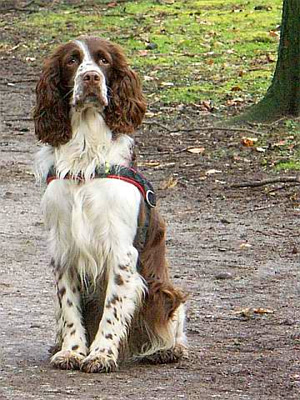
\includegraphics[height=4cm]{spaniel.jpg}
\includegraphics[height=4cm]{wolf.jpg}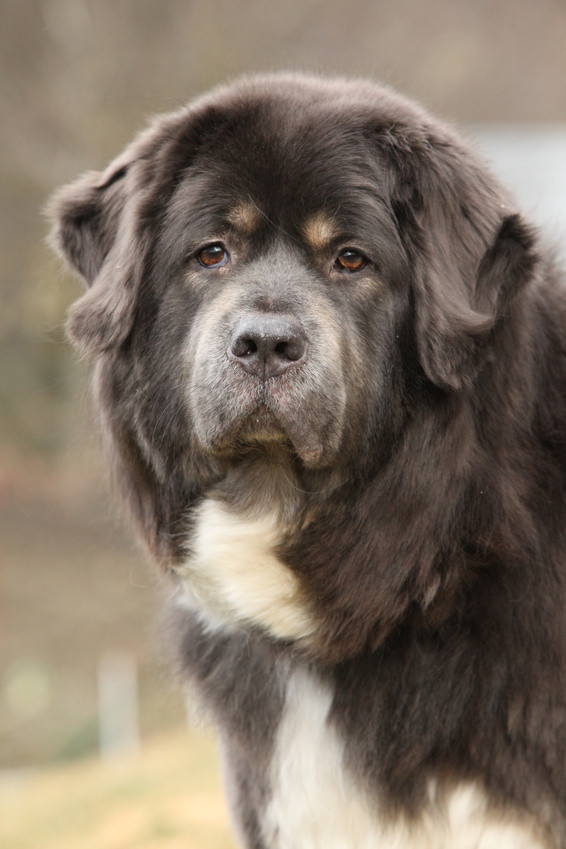
\includegraphics[height=4cm]{mastiff.jpg}
		\caption{Spanjel, hunt ja mastif}
	\end{center}
\end{figure}

Niisiis, koodi ümber kirjutamine on kallis, keeruline ning seotud oluliste riskidega. Samas on olemasoleva rakenduse putitamisel samuti üks oluline puudus: me toimime jätkuvalt kord juba defineeritud arhitektuuri, täpsemalt öeldes kontseptsiooni, raamides. Ehk, asjade ümber kirjutamine annab võimaluse innovatsiooniks ning asjade puhtalt lehelt uuesti mõtestamiseks. Jah, spanjelist on ilmselt võimalik mastifi-laadne elukas aretada aga võibolla on efektiivsem alustada siiski nende ühisest eellasest, hundist? Kindlasti tuleks keskenduda mitte tehnilisele vaid ärilisele innovatsioonile ümber mõtestades äriprotsesse, automatiseerides ning efektiivistades. Seejuures on muidugi eelduseks, et meil on piisavalt aega ja raha seda mõttetööd põhjalikult ette võtta ning et on alust eeldada, et tulemus praegusest olukorrast oluliselt erineb.

Lõpuks tuleb panna kõrvuti süsteemi ümber kirjutamise kulu, olemasoleva muutmise ning mõlema alternatiivi halduskulude nüüdisväärtus. Kui nüüd tundub, et rakenduse uuesti kirjutamine on siiski mõistlik, on oluline aru saada, miks nii läks. Jällegi Joelile toetudes, ei ole mõistlik eeldada, et kui ühel korral ei õnnestunud hankida mõistlikku süsteemi või seda pusaks muutumast hoida, siis teisel korral asjad teisiti lähevad. On oluline, et suudetakse välja tuua konkreetsed tegevused, mille abil hoidutakse vajadusest süsteem uuesti ümber kirjutada. Siinkohal kuuleb ilmselt argumenti \emph{build one to throw away} aga sel juhul peaks olema võimalik vähemalt üles kirjutada, mida esimesest korrast täpselt õpiti.

\TODO:  \cite{nlp}, kontseptsiooni venitamise idee. Kui nii funktsioon kui vorm on arenenud kaugemale algsest kontseptsioonist.

\subsection{Taakvara ja testid}
Taakvara\index{Taakvara} võib määratleda ka tarkvaratehnilisest küljest. \citeauthor{feathers2004working} määratleb taakvara kui lihtsalt testideta koodi. \cite{feathers2004working} Ta arutleb nii: kui koodil ei ole teste, ei saa me teda muuta. Ükskõik kui hästi, puhtalt ja kenasti kood ka kirjutatud ei ole, ei tea me tema käitumisest ilma testideta midagi. Veelgi enam, me ei tea midagi tema \emph{olulisest} käitumisest. Kood võib toimida väga erinevatel viisidel aga ilma testideta ei ole meil võimalik eristada soovitud käitumist soovimatust. Ja kui nii, siis ei ole ilma testideta võimalik hinnata, kas meie kood läheb muutuste järel paremaks või halvemaks. Nii on aga sihipärane koodi muutmine võimatu.

Kui aga koodi muuta ei saa, muutub ta varast kohustuseks. Nii ei ole testimispõhine taakvara definitsioon mitte nii ärikauge, kui algselt paistab: argumentatsiooni juured on ärilise väärtuse\index{Väärtus} lisamises.

\section{Tehniline võlg}
\index{Tehniline võlg}
On kriitiline, et tellija\index{Tellija} saaks aru oma tegevuse tagajärgedest. Mis, arvestades teo ja selle tagajärje ajalist vahet, on väga keeruline. Põhjus on selles, et tehnilise võla likvideerimine tuleb arenduse läbilaskevõime arvelt. Järelikult tähendab tehnilise võla kuhjumine, et arenduse läbilaskevõime ajas kahaneb. Kui tellija ei saa aru, et tema otsus tekitas tehnilise võla, on IT-juhil kaks põhimõttelist otsust. Ta kas keeldub tehnilist võlga tekitamast, näib paindumatu ja lastakse lahti või ta võtab tehnilise võla, asub seda IT võimekust vähendades likvideerima ning ta lastakse lahti. Ehk, häid valikuid ei ole. Järelikult ei ole IT juhil muud valikut peale tellija harimise.

Tehnilise võla oluline aspekt on seotud süsteemi piiride küsimusega. Kuna tehniline võlg on seotud konkreetse süsteemiga kuid, definitsiooni järgi, on süsteemi piirid alati suvalised, võib rääkida tehnilise võla skoobist. On võimalik olukord, kus lokaalsete optimumide saavutamise läbi võetakse süsteemi kui terviku suhtes tehnilist võlga. Näiteks võib ehitada kõik süsteemid tähtajaks kuid mitte arvestades teiste süsteemi osade integratsioonivajadusi. Üksiku süsteemi vaatepunktist võlga ei ole. Süsteem kui tervik aga võib vajada olulist investeeringut oma komponentide suhtluse tagamiseks. 

Tehnilise võla juhtimine on teatavas mõttes sarnane finantsvõla juhtimisega: rahavoogude nüüdisväärtuse abil on võimalik teha otsuseid. Tehnilisel võlal on siiski ka aspekte, mida lihtsasti finantsmudelisse valada ei õnnestu. Teatavast piirist alates hakkab tehniline võlg takistama värbamist ja inimeste hoidmist. Tegemist on raskestivarjatava stressifaktoriga ning üha vähem leidub inimesi, kes \enquote{selle supiga} on nõus tegelema. Nii võib alata lõigus \ref{sec:kokkuhoid} kirjeldatuga sarnane tagasiside, kus kompetentsete inimeste lahkumine viib võla suurenemiseni mis omakorda tõrjub kompetentseid inimesi. 

\section{Tehnilise võla teine külg}
Võlal on alati kaks poolt. Saab võlgu anda ja saab võlgu võtta. Kas tehnilise võlaga on ka nii? Selle koha peal, kardetavasti, saab meie metafoor otsa. Sest päris täpset vastet võla andmisele ei ole. Küll aga võime endale tuleviku ees kohustusi võtta mitte tööd tegemata jättes vaid seda liiga palju tehes\sidenote{Siin suurepärased näited: \url{http://hackingdistributed.com/2016/04/05/how-software-gets-bloated/}}. 

Olgu meil tegu süsteemiga, mis on suur, keeruline ja raskesti muudetav. Sellega toimetavad nutikad ja hästi makstud inimesed. Nutikad ja hästi makstud inimesed suudavad lahendada keerulisi probleeme, seepärast nad hästi makstud ongi. Aga paraku on nutikatel inimestel komme mõnikord ka lihtsaid probleeme natuke keeruliselt lahendada. Ja isegi, kui probleem tõepoolest keerulist lahendust õigustab, tekib küsimus: kas me suudame edaspidi leida piisavalt nutikaid inimesi? Ja kui suudame, siis kas on inimlikult võimalik keeruliste lahenduste kohta käivat teadmust mõistlike kadudega ühest peast teise liigutada? 

Skype kui selline on hea näide sedalaadi keerulisest süsteemist. P2P\index{Skype!P2P} võrk on ülikeeruline ja väga elegantne lahendus keerulisele ärilisele probleemile. Lahenduse hind oli aga, et ainult väike hulk väga häid programmeerijaid suutis tolle võrgu arendamisega tegeleda või isegi sealseid probleeme hoomata. Mõelge näiteks algoritmile, mis suudab paarikümne osalejaga sõnumi-vestluste olekut\sidenote{Sealhulgas nii sõnumid kui ka näiteks lisatud ja eemaldatud osalised. Sõnumeid kirjutada, kasutajaid lisada ja eemaldada jne. on võimalik ka ilma võrguühenduseta. Tegu on ühe eriti keerulist liiki konsensusprotokolliga.} kõigi osapoolte vahel sünkroniseerida. Selle algoritmi kohta oli peamine teadmine ühe inimese peas ning kui too põhjalikku dokumentatsiooni maha jättes lahkus, ei õnnestunudki kogu teadmist üle võtta.

Üks arhitektuuri puhul kehtivatest printsiipidest on, et süsteemi disain ei tohi eeldada kõrgemat tootmisvõimekust, kui planeeritud. Disainides F1 stiilis tolerantsidega mootori ja andes selle toota tavasõidukite mootorite tehasele, ei saa tulemus hea olla. Väga paljud infosüsteemide hädad tulenevad liiga headest arhitektidest, kes loovad efektseid keerulisi süsteeme arvestamata, et neid hakkavad realiseerima täiesti keskmised tavalised programmeerijad. 

Keerukuse kasvu ei saa paraku alati arhitektuursete vahenditega vältida. Programmeerijale jääb reeglina mingi vastutus disainiotsuste üle ja seal võib kergesti olla ruumi äärmiselt keerulistele lahendustele. Kerkinud keerukuse-probleemi lahendamine on reeglina siiski arhitekti ülesanne. 

Jõuame olulise järelduseni, et nii arhitekti töö kui süsteemi jätkusuutlikkus tervikuna sõltuvad mitte ainult kasutatavate programmeerijate kompetentsist vaid ka organisatsiooni võimest seda kompetentsi taset hoida või kasvatada. Järelikult on arhitekti starteegiline huvi mõista asutuse personali- ja koolituspoliitikat.Kui see ebasoovitavas suunas muutuma peaks, tuleb otsustajaid riskidest teavitada kuid kindlasti ka omalt poolt maandamismeetmeid tarvitusele võtta.


\section{Alandlik programmeerija}
\label{humble}
Edsger W. Dijkstra\index{Dijkstra, Edsger W.} on inimene, kes arvuti-inimeste hulgas tutvustamist ei vaja ja kel tiitleid rohkem, kui loetleda jõuab. Muu hulgas on ta 1972. aastal saanud Turingi Auhinna. Nagu kombeks, järgnes auhinnale avalik loeng \citep{yourdon1979classics}, mille pealkirjaks Alandlik Programmeerija. Pika ja tõeliseks nautimiseks mõningast arvutiteaduse tausta vajava jutu peamised teesid on järgmised\footnote{Tõlgitud ja mugandatud aadressilt \url{http://c2.com/cgi/wiki?TheHumbleProgrammer}}:
\begin{itemize}
	\item Kui pürgida töökindla tarkvara ja efektiivse töökorralduse poole, peate leidma viisi vigade vältimiseks nende hilisema otsimise asemel. Selle tulemusena muutub programmeerimine kui protsess odavamaks.
	\item Programmeerijad peaksid tegelema vaid intellektuaalselt hoomatava tarkvaraga
	\item Programmeerijad ei peaks unustama, et nende ülesanne ei ole programmeerida. Nende ülesanne on disainida lahendusi, mis käituvad soovitud viisil
	\item Tavaliselt kirjutatakse programm ja siis seda testitakse. Kuid testimine on paremal juhul efektiivne viis vigade olemasolu tuvastamiseks. Vigade puudumise  tõestamiseks on testimine lootusetu
	\item Kompetentne programmeerija on teadlik oma pea väga piiratud suurusest. Seega läheneb ta programmeerimisülesandele alandlikus meeles ning, muu hulgas, väldib nutikaid trikke nagu katku
	\item Kohmakas tarkvaratehnika on talutav vaid senikaua, kuni riistvara moodustab suurema osa projekti eelarvest
\end{itemize}

\section{Küsimusi aruteluks}
\subsection{Mis teeb programmeerimise keeruliseks?}

Brooks\index{Brooks, Frederick P.} ütleb, et programmeerimine on põhimõtteliselt keeruline\cite{brooks1975mythical}. Ta jagab tarkvaratehnilise keerukuse kaheks, mitteolemuslikuks ja olemuslikuks, ning väidab, et neist esimene on vähendatav ja teine tõenäoliselt mitte. Olemuslik keerukus seisneb peamiselt tarkvara kontseptuaalse mudeli spetsifitseerimises, disainis ja testimises ja mitteolemuslik tolle mudeli võimalikult täpses koodi valamises. 

Kuid Brooks ei seleta väga põhjalikult \emph{miks} töö tarkvara kontseptuaalse mudeliga (mis on sisuliselt seesama, mida me eespool süsteemi kontseptsiooniks nimetasime) põhimõtteliselt keeruline on. Tõenäoliselt on vähemalt üks põhjus arvutite duaalses olemuses. Kogu tänapäevane digitaalne arvutustehnika on üles ehitatud kahevalentsele loogikale. Null ja üks, tõsi ja vale. Täidetakse kas üks koodi haru või teine. Samas pole reaalne maailm sugugi duaalne. Ei leidu ei puhast musta ega valget. Loodus ei tekita ei päris ümmargusi ega päris kandilisi objekte. Ja nii peabki programmeerija suutma konstrueerida mudeli mis ühest küljest peegeldab reaalsuses toimivat ja sellisena ebatäiuslikku äriprotsessi ja teisalt on realiseeritav digitaalarvutiga. Selline tegevus ei ole olemuslikult lineaarne ja tõenäoliselt praeguses tarkvaratehnika paradigmas hästi automatiseeritav ei ole. 

\begin{marginfigure}
		\begin{center}
		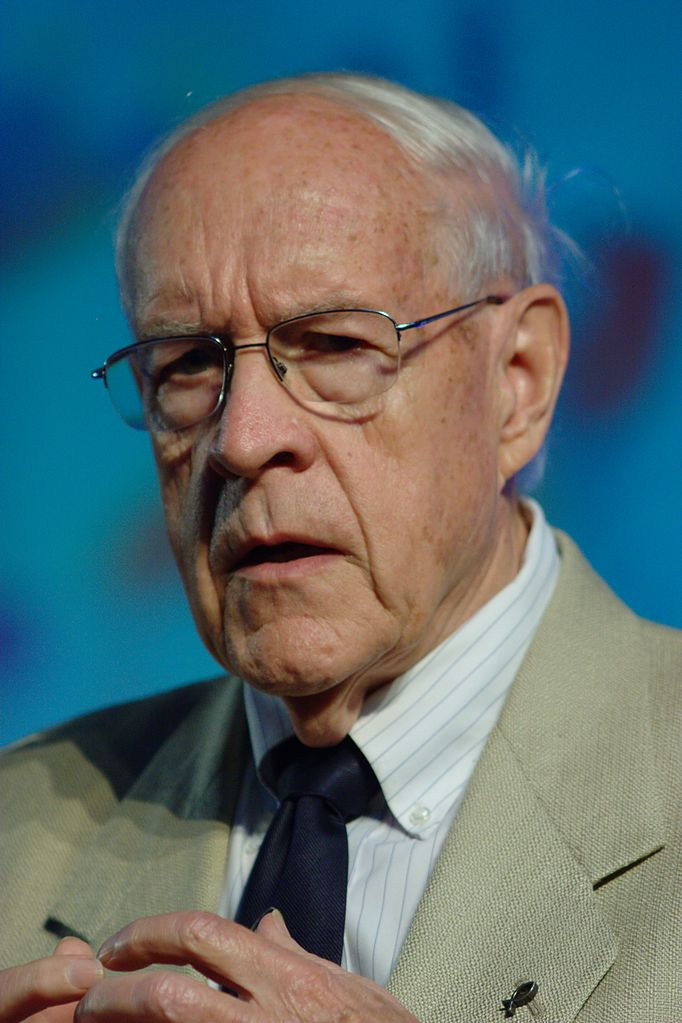
\includegraphics[width=.7\linewidth]{682px-Frederick_Brooks_IMG_2279.jpg}
		\caption{Fred Brooks. Pilt: wikimedia:user:David.Monniaux}
		\label{fig:brooks}
		\end{center}
		Fred Brooks on legendaarne arvutitegelane, kes juhtis IBM\index{IBM} System/360 ja OS/360 arendust. Saadud kogemusest kirjutas ta oma põhiteose, The Mythical Man-Month ning oli hiljem tegev arvutiteadlasena. 
\end{marginfigure}

Kui miski on keeruline, tekitab see kulusid. Kui miski tekitab kulusid, siis on võimalik müüa vahendeid tolle miski vähendamiseks. Ja kuna olemusliku ja mitteolemusliku eristamine mitte lihtne ei ole, siis on läbi ajaloo üritatud üle saada ka tarkvara ehitamise keerukuse probleemist:

\begin{description}
	\item[Nõuete kirjeldamine] Kui me ainult suudaksime nõudeid piisavalt täpselt kirjeldada (ehk oma maailmamudeli võimalikult täpseks ajada), siis on seda võimalik ka üheselt tarkvaras realiseerida. Täna ei leidu vast praktikut, kes sellise väitega nõus oleks. Siiski panustavad mõned metoodikad siiani nõuete ülitäpsesse kirjeldamisse. Mudeli lahutuse tõstmine viib järjest uute detailide esilekerkimiseni mis paratamtult omakorda paljastavad uusi detaile. Kas laud on sile näpuga katsudes, molekuli, aatomi või elektroni tasemel? Äkki peaks rääkima hoopis väljavõrranditest?
	\item[Protsessi järgimine] Kui me ainult suudaksime välja mõelda deterministliku tarkvara loomise protsessi ja panna kõik osapooled seda järgima, peab tulemus olema deterministlik. Paraku ei ole ka parim lineaarne protsess täielik mittelineaarse tegevuse lähend. Nagu ka nõuete juures ilmneb ka parima protsessi puhul järjest uusi nüansse, mida protsessis arvesse võttes paljastub järgmine kiht keerukust
	\item[Artefaktide tootmine] Kui me ainult suudaksime määratleda iga tegevuse täpse tulemi ja sisendi, võiks neid tegevusi vabalt kombineerides saada vähemalt täieliku pildi projektis toimuvast. Ka see tee ei vii suurt kuhugi. Järjest täpsem loova inimese peas toimuva kirjeldamine võtab järjest rohkem aega, viies projekti hilinemiseni, mida ma ju teadupärast lahendame järjest rohkemate ja detailsemalt määratletud artefaktide nõudmise abil
	\item[Protsessist loobumine] Kui me oleme kõike eeltoodut juba proovinud, siis kui me vaid suudaksime kogu selle massi alt programmeerija üles leida ja vabastada, siis hakkaksid ju projektid kohe paremini välja tulema? Selles mõtteviisis on agiilsete meetodite juured. Paraku tavaliselt selgub peagi, et ilma protsessita toimetamine nõuab palju suuremat distsipliini, kui protsessiga ning piiravaks teguriks saab inimeste võimekus omavahel abstraktseid ideid jagada. 
\end{description}

Kõiki neid lahendusi on eri aegadel müüdud kui lahendust tarkvara keerukusele ning ilmsel toob tulevik uusi sedalaadseid. Kuid kuni inimene koodi kirjutab, on ja jääb tarkvara tegemine keeruliseks ning mao-õli müüjatesse tasub suhtuda skepsisega.

\subsection{Kuidas seletada juhtkonnale tehnilist võlga?}
Oma otsuste (eeldades, et võlg on võetud ärilistel põhjustel) tagajärgedega silmtsi seismine ei ole kunagi lihtne\sidenote{Osalt on sellest küsimusest juba eelnevalt räägitud, vt. \nameref{sec:business:q1}}. Põhimõtteliselt on probleem selles, et isegi suhteliselt lihtsa dünaamilise mudeli käitumine ei ole intuitiivne ning lihtsasti mõistetav. \citeauthor{ledet1994manufacturing} on tegelenud keeruliste dünaamiliste mudelitega tootmisettevõtetes\cite{ledet1994manufacturing}. Nad leidsid, et probleemi tuvastamine arvutimudelite abil on suhteliselt lihtne kuid tulemuse presenteerimine viisil, mis ka organisatsioonilise muutuse esile kutsuks, on keerukas. Nad proovisid kolme lähenemisviisi.

Esmalt üritasid nad seletada mudelit, selle eeldusi ning näidata tulemusi. Tulemus oli pettumustvalmistav. Kuna mudeli tulemus on reeglina suhteliselt triviaalne, tekkis tihti küsimus \enquote{kas tõesti pidi mudel teile seda ütlema?} ning eelduste selgitamine oli kõigile osapooltele frustreeriv.

Teiseks presenteeriti mudeli tulemusi seletamata nende saamise viisi. Tegu oli küllalt efektiivse lähenemisega, mille tulemused kergesti omaks võeti. Kuna, jällegi, mudeli tulemus on triviaalne kostis tihti kommentaare stiilis \enquote{ma olen seda juba aastaid rääkinud!}.\sidenote{Tekib siiski küsimus, kust ja miks said analüütikud nende tõsiselt võtmiseks piisava usalduskrediidi}

Kolmandaks loodi simulatsioonimäng ja mängiti see multidistsiplinaarse meeskonnaga ka läbi. Nii oli osalistel võimalik mitte ainult modelleerimise tulemust näha vaid selleni ka iseseisvalt ja ohutus keskkonnas jõuda. 

Sarnaste tulemusteni on jõutud ka mujal. MIT Sloan School of Management uurijad arendasid kuuekümnendatel välja \enquote{õllemängu}\cite{sterman1984instructions}. Mängu mõte on demonstreerida osalistele ka lihtsate tarneahelate kõrget dünaamilist keerukust ning võimaldada kasutada erinevaid sellega toime tuleku strateegiaid. Mängus osalejad simuleerivad poest, hulgimüüjast ja tootjast koosnevat õlle tarneahelat, kus iga sammu vahel on ajaline nihe. Tuleb välja, et ka mõne käigu kaugusele ulatuv vahe põhjuse ja tagajärje vahel ei ole lihtsasti hoomatav ning osapooled kipuvad kergesti pankrotti minema. Seda ka pärast põhjalikku mängu ja tema olemusega tutvumist. 

Ehk, tulles tagasi algse probleemipüstituse juurde, ei ole juhkonnale tehnilise võla selgitamine lihtne ülesanne. Enamasti ei ole IT juhi kästuses ei mänguvõimalust ega ka modellerimisvõimekust. Mida tavaliselt siiski teha õnnestub, on tehnilise võla läbipaistvaks muutmine näiteks arendussaba\index{Arendussaba} nähtavaks muutmise läbi. Seda saab omakorda teha tavalise veahaldustarkvara abil. Oluline on silmas pidada, et too saba siis ka tõesti soetud oleks ning sisaldaks igal hetkel selgelt markeerituna asju, mida on eksplitsiitselt otsustatud mitte teha. 
